\documentclass{article}

\usepackage{amsmath}

\usepackage{graphicx}
\graphicspath{ {../outputs/} }

\usepackage[style=numeric, backend=bibtex8]{biblatex}
\addbibresource{citations.bib}

\begin{document}

  \title{Linear Time Generation of Simulated Wireless Sensor Networks with Random Geometric Graphs}
  \author{Luke Wood}
  \maketitle

  \section{Executive Summary}
  \subsection{Introduction and Summary}
	Wireless Sensor Networks can be incredibly expensive to deploy and test which makes them an excellent candidate for simulated testing.
	Vlady Ravelomananana and Hichem Kenniche from the University of Paris first explored the concept of using random geometric graphs (RGGs) to attempt to model wireless sensor networks \cite{kenniche2010random}.
	RGGs can be used as a relatively cheap way to gather valuable information about how wireless sensor networks can function and communicate.
	Through a series of reports	I will be:
	\begin{enumerate}
		\item Generating RGGs on the geometries of a unit square, unit disc, and unit sphere
		\item Color the generated graph in linear time using smallest vertex last ordering (TODO check)
		\item Find the terminal clique in the generated RGGs
		\item Find a selection of bipartite subgraphs producted by an algorithm for coloring
	\end{enumerate}
	This report is the first of the series and  will describe an implementation for a linear time algorithm to generate graphs consisting of N vertices with an average degree of A on the geometric topologies of: unit square, unit disc, unit sphere.

	\begin{tabular}{ |c|c|c| }

	\end{tabular}

  \subsection{Programming Environment Description}
  	The implementation of the algorithm used to gather the data supporting this report was gathered on a 15 inch Macbook pro 2017 with a 2.9 GHz Intel Core i7 processor and 16 GB of RAM.

  \section{Reduction to Practice}

  In order to ensure that average degree of the nodes is close to the desired average degree we define a radius surrounding each node.
  The formulas to find the radius for each topology is derived from the equations found in the paper Bipartite Grid Partitioning of a Random Geometric Graph\cite{chen2017bipartite}.
  The formula used to find this radius varies for each graph tolopogy and can be found in the table displayed below:

  \begin{tabular}{ |c|c|c| }
	  \hline
	  Topology & Equation in Chen's Paper & Equation for Radius Derive from Chen's \\
	  \hline
	  Unit Square & $d(G) \approx N\pi r^2 $ & $r = sqrt(\dfrac{d(G)}{N\pi})$ \\
	  \hline
	  Unit Disc   & & \\
	  \hline
	  Unit Sphere & & \\
	  \hline
  \end{tabular}

  \begin{figure}[!htb]
    \centering
    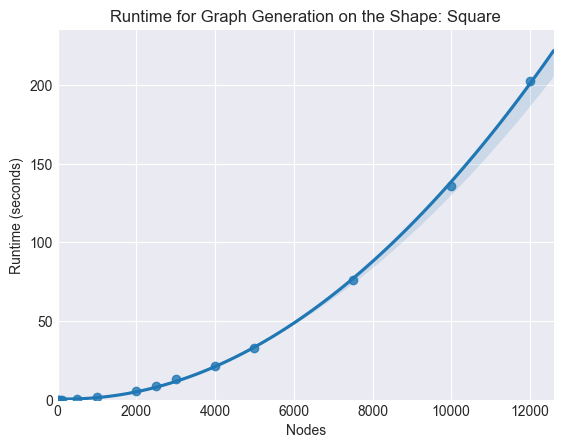
\includegraphics[width=1 \textwidth]{square/runtime/runtime_chart_naive}
    \caption{Data on the Runtime of the $O(n^2)$ Algorithm}
  \end{figure}

  \begin{figure}[!htb]
    \centering
    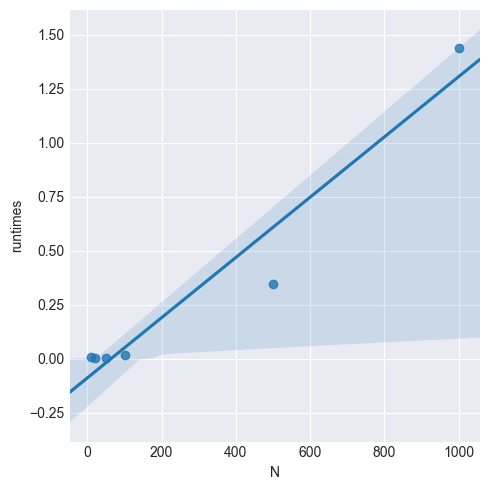
\includegraphics[width=1 \textwidth]{square/runtime/runtime_chart}
    \caption{Data on the Runtime of the $O(n)$ Algorithm}
  \end{figure}

\section{Result Summary}
  The algorithm I created is clearly $O(n)$

\printbibliography

\end{document}
